% Created 2017-05-08 Mon 09:16
\documentclass{beamer}
\usepackage{fixltx2e}
\usepackage{graphicx}
\usepackage{longtable}
\usepackage{float}
\usepackage{wrapfig}
\usepackage{soul}
\usepackage{textcomp}
\usepackage{marvosym}
\usepackage{wasysym}
\usepackage{latexsym}
\usepackage{amssymb}
\usepackage{hyperref}
\tolerance=1000
\usepackage{etex}
\usepackage{amsmath}
\usepackage{pstricks}
\usepackage{pgfplots}
\usepackage{tikz}
\usepackage[europeanresistors,americaninductors]{circuitikz}
\usepackage{colortbl}
\usepackage{yfonts}
\usetikzlibrary{shapes,arrows}
\usetikzlibrary{positioning}
\usetikzlibrary{arrows,shapes}
\usetikzlibrary{intersections}
\usetikzlibrary{calc,patterns,decorations.pathmorphing,decorations.markings}
\usepackage[BoldFont,SlantFont,CJKchecksingle]{xeCJK}
\setCJKmainfont[BoldFont=Evermore Hei]{Evermore Kai}
\setCJKmonofont{Evermore Kai}
\usepackage{pst-node}
\usepackage{pst-plot}
\psset{unit=5mm}
\usepackage{beamerarticle}
\mode<beamer>{\usetheme{Frankfurt}}
\mode<beamer>{\usecolortheme{dove}}
\mode<article>{\hypersetup{colorlinks=true,pdfborder={0 0 0}}}
\AtBeginSection[]{\begin{frame}<beamer>\frametitle{Topic}\tableofcontents[currentsection]\end{frame}}
\setbeamercovered{transparent}
\providecommand{\alert}[1]{\textbf{#1}}

\title{数字图像处理绪论}
\author{}
\date{}
\hypersetup{
  pdfkeywords={},
  pdfsubject={},
  pdfcreator={Emacs Org-mode version 7.9.3f}}

\begin{document}

\maketitle

\begin{frame}
\frametitle{Outline}
\setcounter{tocdepth}{3}
\tableofcontents
\end{frame}













\section{数字图像处理的概念}
\label{sec-1}
\begin{frame}
\frametitle{数字图像处理}
\label{sec-1-1}
\begin{block}{什么是数字图像处理}
\label{sec-1-1-1}

数字图像处理(Digital Image Processing)又称为计算机图像处理,它是指将图像信号转换成数字信号并利用计算机对其进行处理的过程。
\end{block}
\end{frame}
\begin{frame}
\frametitle{数字图像特点}
\label{sec-1-2}

\begin{itemize}
\item 数字图像,又称数码图像或数位图像,是二维图像用有限数字数值像素的表示。
\item 由数组或矩阵表示,其光照位置和强度都是离散的。
\item 数字图像是由模拟图像数字化得到的、以像素为基本元素的、可以用数字计算机或数字电路存储和处理的图像。
\end{itemize}
\end{frame}
\begin{frame}[fragile]
\frametitle{数字图像示例}
\label{sec-1-3}
\begin{columns}
\begin{column}{0.5\textwidth}
\begin{block}{图像}
\label{sec-1-3-1}

\includegraphics[width=\textwidth]{./image/a.png}
\end{block}
\end{column}
\begin{column}{0.5\textwidth}
\begin{block}{内容}
\label{sec-1-3-2}


\begin{verbatim}
 72  208   93  106  212
  2   73   69  178  234
 18  228  244   99   75
223  245  221  100   52
 84  239  238  105   69
\end{verbatim}
\end{block}
\end{column}
\end{columns}
\end{frame}
\begin{frame}
\frametitle{数字图像类别}
\label{sec-1-4}

\begin{itemize}
\item 二值图像 (Binary Image): 图像中每个像素的亮度值(Intensity)仅可以取自0到1的图像。
\item 灰度图像 (Gray Scale Image),也称为灰阶图像: 图像中每个像素可以由0(黑)到255(白)的亮度值表示。0-255之间表示不同的灰度级。
\item 彩色图像 (Color Image):每幅彩色图像是由三幅不同颜色的灰度图像组合而成,一个为红色,一个为绿色,另一个为蓝色。
\item 伪彩色图像(false-color)
\item 多光谱图像(multi-spectral thematic )
\item 立体图像 (Stereo Image):立体图像是一物体由不同角度拍摄的一对图像,通常情况下我们可以用立体像计算出图像的深度信息。
\item 三维图像 (3D Image):三维图像是由一组堆栈的二维图像组成。每一幅图像表示该物体的一个横截面。
\end{itemize}
\end{frame}
\begin{frame}
\frametitle{数字图像存储格式}
\label{sec-1-5}

\begin{itemize}
\item BMP
\item JPG
\item PNG
\item GIF
\item TIFF
\item Netpbm
\end{itemize}
\end{frame}
\begin{frame}
\frametitle{课程主要内容}
\label{sec-1-6}


\begin{itemize}
\item 数字图像基础
\item 空间域图像增强
\item 频率域图像增强
\item 图像复原
\item 彩色图像处理
\item 图像分割
\item 目标识别
\end{itemize}
\end{frame}
\begin{frame}
\frametitle{与其它课程关系}
\label{sec-1-7}


\begin{itemize}
\item 模式识别
\item 机器视觉
\item 最优化理论与方法
\item 控制理论
\item 生物学
\item 心理学
\item 哲学
\end{itemize}
\end{frame}
\begin{frame}
\frametitle{数字图像处理历史}
\label{sec-1-8}

\begin{itemize}
\item Bartlane cable picture transmission system, 1920s
\item improve images from a space probe, JPL, 1964
\item Computerized tomography(CT), 1970s
\end{itemize}
\end{frame}
\section{数字图像处理应用}
\label{sec-2}
\begin{frame}
\frametitle{数字图像处理示例}
\label{sec-2-1}

\begin{itemize}
\item 无人驾驶汽车
\item 手写识别
\item 人脸识别
\end{itemize}
\end{frame}
\begin{frame}
\frametitle{ALVINN [Pomerleau] drives 70 mph on highways}
\label{sec-2-2}


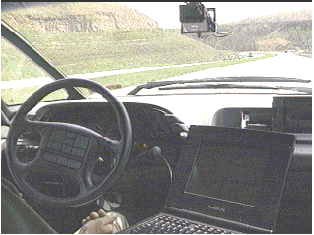
\includegraphics[width=0.3\textwidth]{./image/nl5-interior-front-color.png}
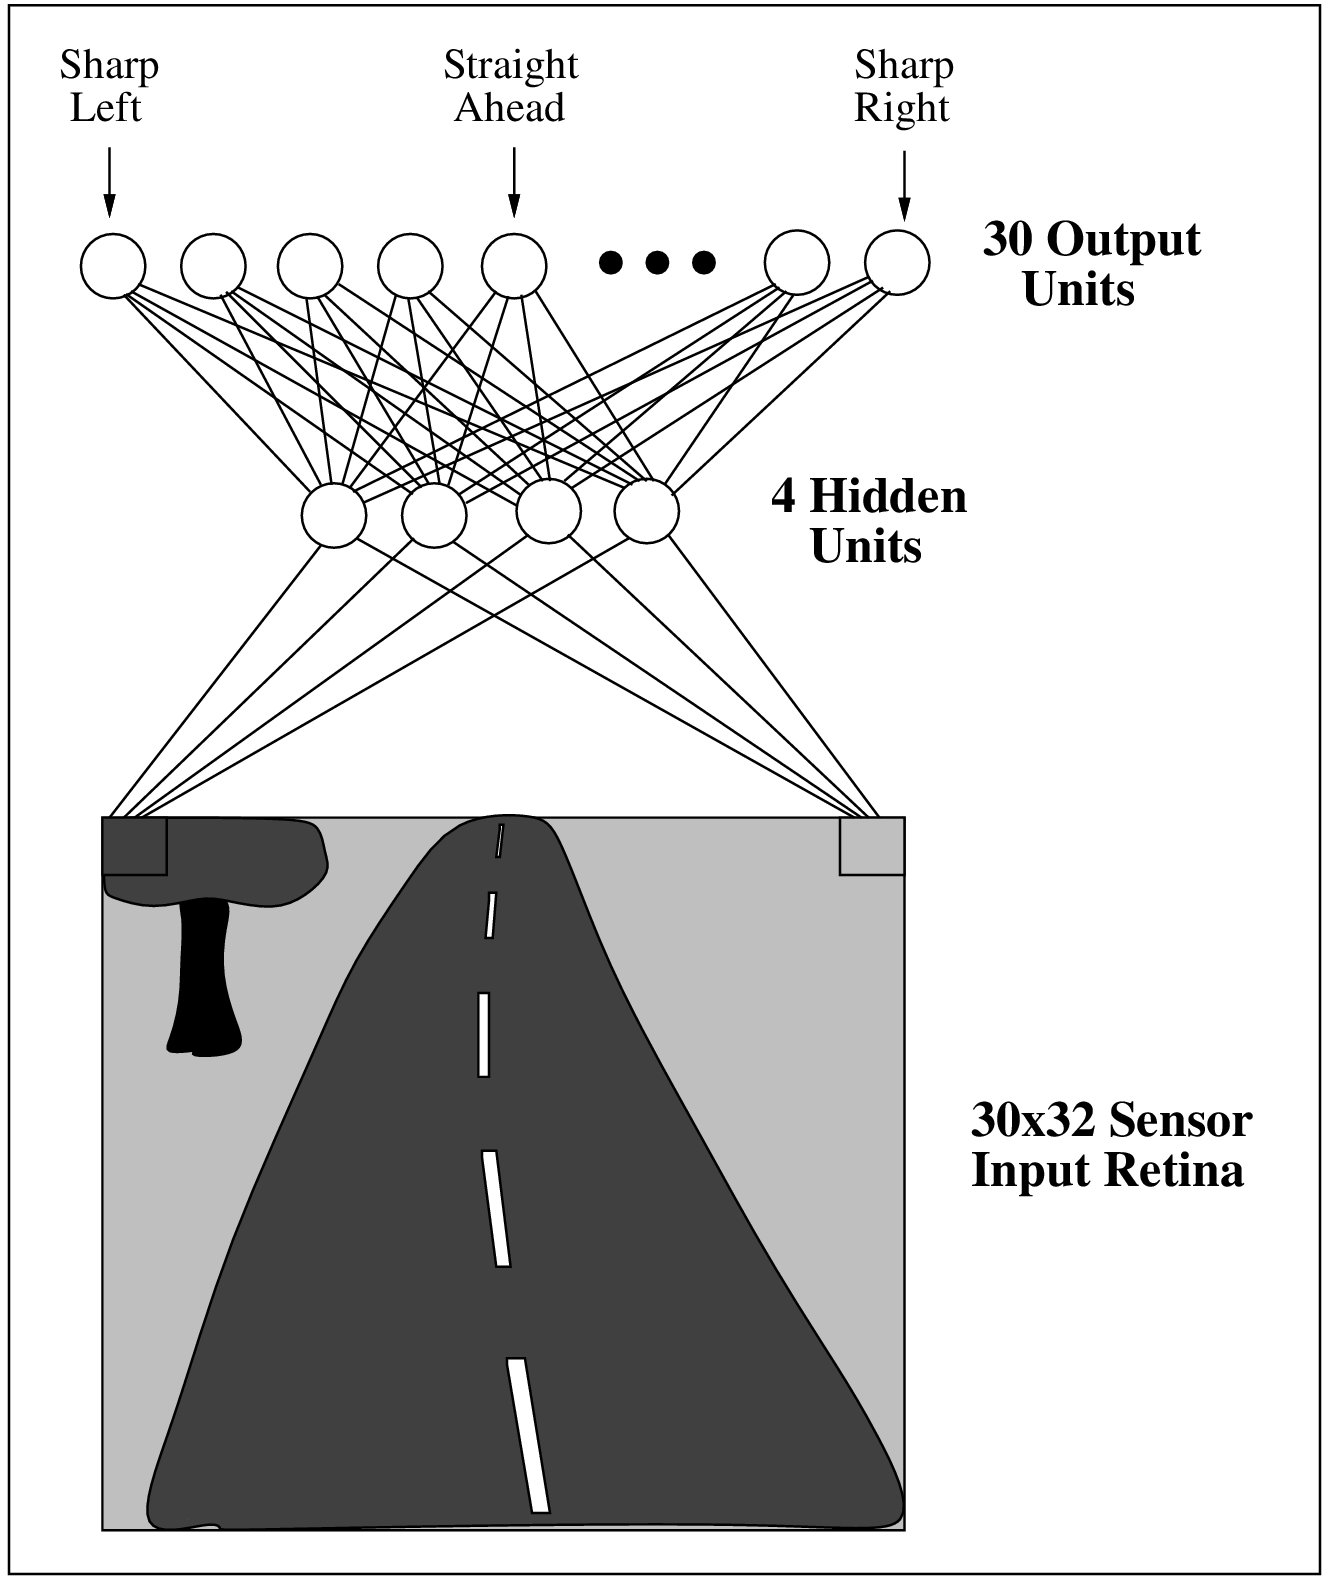
\includegraphics[width=0.3\textwidth]{./image/alvinn1.png}
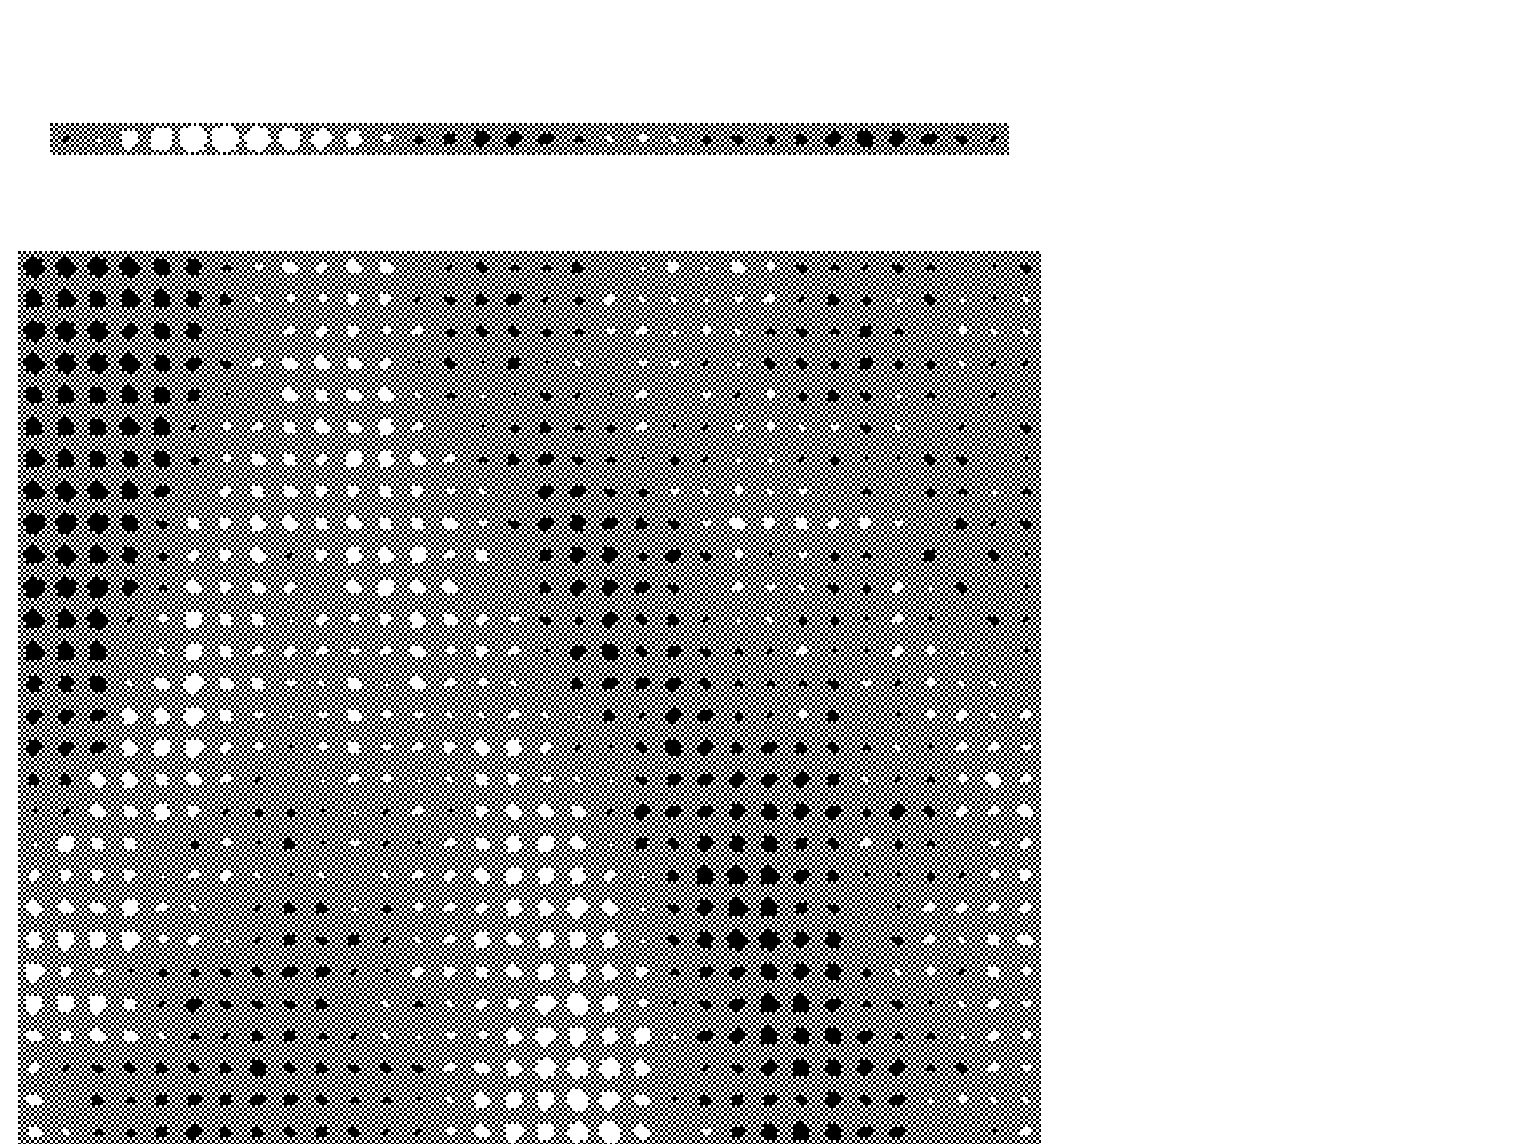
\includegraphics[width=0.3\textwidth]{./image/alvinn2.png}
\end{frame}
\section{数字图像处理技术}
\label{sec-3}
\begin{frame}
\frametitle{数字图像处理的基本内容}
\label{sec-3-1}

\begin{itemize}
\item 图像获取
\item 图像增强
\item 图像恢复
\item 彩色图像处理
\item 图像压缩
\item 形态学处理
\item 图像分割
\item 表示与描述
\item 识别
\end{itemize}
\end{frame}
\begin{frame}
\frametitle{数字图像处理系统的组成}
\label{sec-3-2}

\begin{itemize}
\item 传感器
\item 专用图像处理器件
\item 通用计算器件
\item 图像处理软件
\item 存储器
\item 显示器
\item 网络
\end{itemize}
\end{frame}
\section{数字图像处理相关资源}
\label{sec-4}
\begin{frame}
\frametitle{课程}
\label{sec-4-1}

\begin{itemize}
\item \href{https://www.coursera.org/learn/digital}{https://www.coursera.org/learn/digital}  Fundamentals of Digital Image and Video Processing(coursera)
\item \href{https://www.coursera.org/learn/image-processing}{https://www.coursera.org/learn/image-processing}  Image and Video Processing: From Mars to Hollywood with a Stop at the Hospital(coursera)
\item \href{https://www.coursera.org/learn/machine-learning}{https://www.coursera.org/learn/machine-learning}  Machine Learning Stanford University (coursera)
\item \href{http://open.163.com/special/opencourse/machinelearning.html}{http://open.163.com/special/opencourse/machinelearning.html}  斯坦福大学公开课 :机器学习课程(网易公开课)
\item \href{http://open.163.com/special/opencourse/learningfromdata.html}{http://open.163.com/special/opencourse/learningfromdata.html} 加州理工学院公开课:机器学习与数据挖掘
\end{itemize}
\end{frame}
\begin{frame}
\frametitle{资料}
\label{sec-4-2}

\begin{itemize}
\item \href{https://www.kaggle.com/}{https://www.kaggle.com/}
    数据科学竞赛平台、社区
\item \href{http://philschatz.com/biology-book/}{http://philschatz.com/biology-book/}  
    a  freedom book about biology
\item \href{http://www.cs.cmu.edu/~tom/mlbook-chapter-slides.html}{http://www.cs.cmu.edu/\textasciitilde tom/mlbook-chapter-slides.html}
    Machine Learning slide (\LaTeX{} source )
\item \href{http://www.cs.cmu.edu/afs/cs.cmu.edu/project/theo-20/www/mlbook/latex-support.html}{http://www.cs.cmu.edu/afs/cs.cmu.edu/project/theo-20/www/mlbook/latex-support.html} 
    Machine Learning slide (\LaTeX{} source )
\item \href{https://learnxinyminutes.com}{https://learnxinyminutes.com}  \textbackslash{}
    各种程序设计语言快速入门
\item \href{http://cos.name/}{http://cos.name/}
    统计技术社区
\item \href{https://databricks.com/}{https://databricks.com/}
    Spark在线学习
\end{itemize}
\end{frame}
\section{工具}
\label{sec-5}
\begin{frame}
\frametitle{图像处理工具}
\label{sec-5-1}

\begin{itemize}
\item GIMP(GNU Image Manipulation Program):  \href{http://www.gimp.org}{http://www.gimp.org}
\item ImageMagick:  \href{http://www.imagemagick.org/script/index.php}{http://www.imagemagick.org/script/index.php}
\item ImageJ:   \href{https://imagej.nih.gov/ij/}{https://imagej.nih.gov/ij/}
\item VLFEET: \href{http://www.vlfeat.org/}{http://www.vlfeat.org/}
\end{itemize}
\end{frame}
\begin{frame}
\frametitle{C/C++}
\label{sec-5-2}

\begin{itemize}
\item \href{http://opencv.org/}{http://opencv.org/}
\item \href{http://cimg.org}{http://cimg.org}
\item \href{http://dlib.net}{http://dlib.net}
\item \href{http://mlpack.org/}{http://mlpack.org/}
\item \href{http://caffe.berkeleyvision.org}{http://caffe.berkeleyvision.org}
\item \href{http://mxnet.io/}{http://mxnet.io/}
\end{itemize}
\end{frame}
\begin{frame}
\frametitle{Lua}
\label{sec-5-3}

\begin{itemize}
\item \href{http://torch.ch}{http://torch.ch}
\item \href{https://github.com/torchnet/}{https://github.com/torchnet/}
\end{itemize}
\end{frame}
\begin{frame}
\frametitle{Python}
\label{sec-5-4}

\begin{itemize}
\item \href{http://scikit-learn.org/}{http://scikit-learn.org/}
\item \href{http://scikit-image.org/}{http://scikit-image.org/}
\item \href{https://www.tensorflow.org}{https://www.tensorflow.org}
\item \href{http://www.deeplearning.net/software/theano/}{http://www.deeplearning.net/software/theano/}
\item \href{https://github.com/NervanaSystems/neon}{https://github.com/NervanaSystems/neon}
\end{itemize}
\end{frame}
\begin{frame}
\frametitle{Java}
\label{sec-5-5}

\begin{itemize}
\item \href{https://imagej.nih.gov/ij/}{https://imagej.nih.gov/ij/}
\item \href{http://www.cs.waikato.ac.nz/ml/weka/index.html}{http://www.cs.waikato.ac.nz/ml/weka/index.html}
\item \href{http://moa.cms.waikato.ac.nz/}{http://moa.cms.waikato.ac.nz/}
\item \href{http://spark.apache.org/mllib/}{http://spark.apache.org/mllib/}
\item \href{https://mahout.apache.org/}{https://mahout.apache.org/}
\item \href{http://www.h2o.ai/}{http://www.h2o.ai/}
\item \href{http://deeplearning4j.org/}{http://deeplearning4j.org/}
\item \href{http://neuroph.sourceforge.net/}{http://neuroph.sourceforge.net/}
\item \href{http://airbnb.io/aerosolve/}{http://airbnb.io/aerosolve/}
\end{itemize}
\end{frame}
\begin{frame}
\frametitle{科学计算}
\label{sec-5-6}

\begin{itemize}
\item R(Rstudio)
\begin{itemize}
\item R \href{https://www.r-project.org/}{https://www.r-project.org/}
\item Rstudio(R)  \href{https://www.rstudio.com/}{https://www.rstudio.com/}
\end{itemize}
\item Matlab/Octave
\item Scilab
\item Sage
\item Julia
\item Spyder(Python)
\item RapidMiner \href{https://rapidminer.com/}{https://rapidminer.com/}
\end{itemize}
\end{frame}

\end{document}
